\subsection{Mari0: Mario Bros con portales}

Tal y como hemos explicado anteriormente, este videojuego es la combinación entre los miticos Mario Bros y P0rtal. Al ser una combinación entre estos videojuegos comparte muchos de sus elementos, entre ellos su objetivo. El objetivo de estos videojuegos es llegar al final de cada nivel. En cada nivel se proponen diferentes retos y usando los elementos del entorno disponibles y las mecanicas propias del juego, se deben resolver estos retos. El juego está limitado a 4 jugadores como máximo.

\subsubsection{Mecanicas}

Las mecanicas pricipales de este juego son el movimiento basico del Mario y la pistola de portales. El movimiento basico consiste en el movimiento a izquierda o derecha y el salto. La pistola de portales es algo más compleja. 

\subsubsection*{Movimiento y acciones}

El movimiento y las acciones basicas de este juego son más variadas que en juegos similares. Algunas de estas acciones no se han implementado en el entorno porque añadian demasiada complejidad al entorno o simplemente porque no añadian ninguna ventaja. Las pricipales acciones que se pueden realizar son:

\begin{itemize}
    \item Movimiento: Moverse a la derecha o izquierda.
    \item Sprint: cuando se esta moviendo hacia alguna direccion es posible esprintar. Esta accion no está implementada en el entorno.
    \item Salto alto: Este es el salto en el cual se llega a maxima altura. Este es el unico tipo de salto que esta implementado en el entorno.
    \item Salto bajo: Si una vez presionado el boton de salto, se deja de presionar, el jugador realiza un salto de menor altura. Este tipo de salto no está implementado.
    \item Usar objeto: Esta accion usa el objeto que esta más cerca del jugador. Se usa principalmente para agarrar cajas y accionar pulsadores.
    \item Ataque: Esta accion solo puede usarse cuando el jugador esta en el estado de Mario de fuego. El jugador suelta una bolita de fuego que rebota y daña a los enemigos que golpee. Esta accion no esta implementada en el entorno.
    \item Portal 1 y 2: Con esta accion el jugador dispara su portal 1 o 2 en un angulo desde su posición.
    \item Recargar portales: Con esta accion el jugador retira todos los portales que haya colocado.
\end{itemize}

\subsubsection*{Portales}

Cada jugador dispone de una pistola con dos tipos de portales, el portal izquierdo y el derecho o portales 1 y 2, cada uno representado con un color distinto. Estos portales se pueden atravesar por los todos los jugadores y por otros elementos como cajas y laseres. En la figura \ref {fig:portal} podemos ver mejor el funcionamiento de un portal.

\begin{figure}[h]
    \centering
    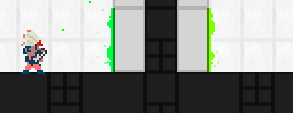
\includegraphics[width=0.9\textwidth]{img/portal-function.png}
    \caption{Funcionamiento de un portal [Elaboración Propia]}
    \label{fig:portal}
\end{figure}

Si el jugador que aparece en la figura atraviesa uno de los lados del portal, aparecerá en el otro lado del portal manteniendo la dirección del movimiento y su velocidad. Extrapolando este conocimiento, cuando un jugador atraviesa un portal, la magnitud de su velocidad se mantendrá intacta al salir por el otro lado del portal, mientras que su dirección estará dictada por la dirección en la que está enfocada el portal de salida.

Aunque los portales son una gran herramienta, tambien tienen sus limitaciones. Las principales limitaciones que hemos encontrado son:

\begin{itemize}
    \item Los portales solo pueden colocarse sobre superficies de color grisaceo como la que podemos ver en la figura anterior.
    \item No es posible disparar proyectiles de portales a traves de un portal abierto.
    \item Cada jugador solo puede tener colocado unicamente 1 portal de cada tipo a la vez. Además, los proyectiles de los portales viajan unicamente en linea recta.
    \item Existen algunos elementos que no permiten que los proyectiles de portales los atraviesen y cuando un usuario pasa a traves de estos, todos los portales colocados por este jugador se eliminan. Adicionalmente, el jugador dispone de una tecla para eliminar todos los portales colocados voluntariamente.
\end{itemize}


\subsubsection{Elementos del entorno}

\subsubsection*{Laseres azules}

Estos laseres son tangibles por los jugadores y por lo tanto pueden servir como platarma o como obstaculo. Adicionalmente, estos laseres pueden atravesar portales dandoles mucha más utilidad. Finalmente, los proyectiles de portales pueden atravesar estos laseres sin sufrir ninguna consecuencia. En la figura \ref {fig:laser-azul} podemos ver un ejemplo de estos laseres.

\begin{figure}[h]
    \centering
    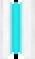
\includegraphics[width=0.1\textwidth]{img/laser-azul.png}
    \caption{Laser azul de Mari0 [Elaboración Propia]}
    \label{fig:laser-azul}
\end{figure}

\subsubsection*{Laseres anti-portales}

Estos laseres son elementos que los jugadores pueden atravesar pero con ciertas consecuencias. En primer lugar, los proyectiles de portales no pueden atravesar estos laseres. Adicionalmente, cuando un jugador los atraviesa, eliminan todos los portales colocados por este jugador. Este laser es muy util en la creacion de niveles y sobretodo para prevenir situaciones extrañas donde un jugador sea teletrasportado a una parte del nivel que ya se haya superado.

\begin{figure}[h]
    \centering
    
\includegraphics[width=0.1\textwidth]{img/laser-antiportal.png}
    \caption{Laser antiportal de Mari0 [Elaboración Propia]}
    \label{fig:antiportal}
\end{figure}

\subsubsection*{Elementos accionadores}

Dentro del entorno existen varios elementos que se pueden accionar, desencadenando así una accion. Los elementos más comunes son botones y pulsadores. Los primeros se accionan cuando tienen un jugador o una caja encima de ellos mientras que los ultimos se accionan mediante la tecla de uso del jugador. Ambos disponen a su vez de una linea que sirve para indicar que elemento accionan. Podemos ver ejemplos de estos elementos en las figura \ref {fig:boton}.

\begin{figure}[h]
    \centering
    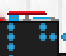
\includegraphics[width=0.1\textwidth]{img/boton.png}
    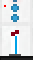
\includegraphics[width=0.05\textwidth]{img/pulsador.png}
    \caption{Boton  y pulsador de Mari0 [Elaboración Propia]}
    \label{fig:boton}
\end{figure}

Además de estos elementos que hemos explicado, existen muchos otros como los geles, cajas, laseres rojos, palancas de salto, laseres anti-gravitatorios etc. El objetivo de este apartado no es explicar todos los elementos que existen si no solo los pricipales. Con los elementos que hemos explicado hasta ahora es suficiente para continuar nuesta explicación del diseño del entorno. 

